 \section{Adding Bibliography}
 
\begin{itemize}
	\item Menurut Wikipedia \par

LaTeX adalah bahasa markup atau sistem penyiapan dokumen untuk peranti lunak TeX. Tex merupakan program komputer yang digunakan untuk membuat typesetting suatu dokumen, atau membuat formula matematika. LaTeX memungkinkan penulis/penggunanya untuk melakukan typesetting dan mencetak hasil kerjanya dalam bentuk tipografi yag terbaik. Oleh karenanya LaTeX paling banyak digunakan oleh para matematikawan, ilmuwan, insinyur, akademisi, dan profesional lainnya.\par

	\item Secara Umum\par

LaTeX adalah word processor (pengolah kata, pembuat dokumen) mirip Microsoft Word. LaTeX lebih cocok digunakan untuk membuat dokumen yang panjang, bukan yang pendek. Dengan begitu, keampuhan LaTeX dapat ditampilkan. LaTeX juga lebih dapat menampilkan kecanggihannya ketika kita menulis scientific document.\par
\vspace{\baselineskip}

\begin{itemize}
	\item Latex
\end{itemize}
 \begin{figure}[ht]
	\centerline{\includegraphics[width=0.70\textwidth]{gambar/Latex}}
	\caption{Latex}
	\label{Latex}
\end{figure}

LATEX adalah alat yang hebat untuk membuat dokumen, ini berdasarkan gagasan wysiwym (what you see is what you mean), idea -> apa yang anda lihat adalah apa yang anda maksud), artinya kita hanya fokus pada isi dokumen saja dan computer yang akan mengurus formatnya. Dengan LATEX sangat mudah untuk membuat bahan yang tampak profesional. \par

\begin{itemize}
	\item Manajemen bibliografi dengan bibtex
\end{itemize}\par


\noindent LATEX mendukung bibliografi, baik membuat referensi dalam dokumen atau menyimpannya dalam file eksternal. Artikel ini menjelaskan bagaimana mengelola bibliografi dengan thebibliography dan sistem BibTeX.\par

\vspace{\baselineskip}
\noindent Catatan: Jika Anda memulai dari nol sebaiknya menggunakan biblatex karena paket tersebut menyediakan pelokalan dalam beberapa bahasa, ini dikembangkan secara aktif dan membuat manajemen bibliografi lebih mudah dan fleksibel.\par

\vspace{\baselineskip}
\noindent Artikel ini menyajikan dasar-dasar untuk membuat dokumen.\par
\vspace{\baselineskip}

\noindent \hspace*{0.5in}Isi\par


\noindent \hspace*{0.5in}1. Perkenalan\par


\noindent \hspace*{0.5in}2 Sistem\par


\noindent \hspace*{0.5in}3 Manajemen bibliografi dengan Bibtex\par


\noindent \hspace*{0.5in}4 Berkas bibliografi\par


\noindent \hspace*{0.5in}5 Menambahkan bibliografi dalam daftar isi\par


\noindent \hspace*{0.5in}6 Panduan Referensi\par


\noindent \hspace*{0.5in}7 Bacaan lebih lanjut\par
\vspace{\baselineskip}
\vspace{12pt}
	\item {\fontsize{14pt}{14pt}\selectfont \textbf{Pengantar/Perkenalan}}\par
\vspace{\baselineskip}
Pengantar\par
Perintah bibliografi standar di LATEX memiliki sintaks yang sama dengan daftar dan item.$\setminus$begin$ \{ $thebibliography$ \} $$ \{ $9$ \} $\par
\begin{verbatim}

\begin{thebibliography}{9}
\bibitem{latexcompanion} 
Michel Goossens, Frank Mittelbach, and Alexander Samarin. 
\textit{The \LaTeX\ Companion}. 
Addison-Wesley, Reading, Massachusetts, 1993.

\bibitem{einstein} 
Albert Einstein. 
\textit{Zur Elektrodynamik bewegter K{\"o}rper}. (German) 
[\textit{On the electrodynamics of moving bodies}]. 
Annalen der Physik, 322(10):891–921, 1905.

\bibitem{knuthwebsite} 
Knuth: Computers and Typesetting,
\\\texttt{http://www-cs-faculty.stanford.edu/\~{}uno/abcde.html}
\end{thebibliography}
\end{verbatim}


Pada thebibliography ini menghasilkan daftar referensi; daftar tersebut akan diberi judul "Referensi" di kelas dokumen artikel, dan "Bibliografi" di kelas buku dan laporan. Parameter di dalam tanda kurung, 9 pada contoh, menunjukkan jumlah entri yang akan ditambahkan; parameter dan ini tidak boleh lebih besar dari 99.\par
Untuk membuat daftar bibliografi, perintah $\setminus$ bibitem ini lah yang digunakan. Parameter di dalam tanda kurung diatur untuk memberi label pada entri tersebut dan nantinya dapat digunakan sebagai pengenal untuk referensi. Setelah penutup, teks dengan nama penulis, judul buku, penerbit dan sebagainya sudah masuk.\par

\begin{figure}[ht]
	\centerline{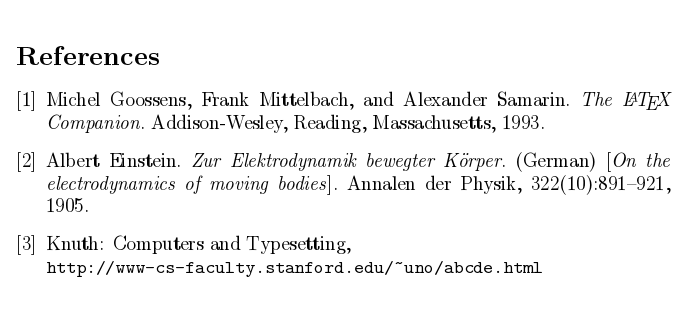
\includegraphics[width=0.70\textwidth]{gambar/Adding}}
	\caption{Daftar Referensi}
	\label{Daftar Referensi}
\end{figure}

\vspace{\baselineskip}
\vspace{12pt}
	\item {\fontsize{14pt}{14pt}\selectfont \textbf{Sistem Tertanam}}\par
\vspace{\baselineskip}
Contoh yang disajikan dalam pendahuluan hanya berisi daftar referensi, contoh berikut menunjukkan bagaimana mengutip entri daftar itu di dalam dokumen.\par

\hspace*{0.5in}$\setminus$begin$ \{ $document$ \} $ \par

\hspace*{0.5in}$\setminus$section$ \{ $First section$ \} $\par

\hspace*{0.5in}This document is an example of $\setminus$texttt$ \{ $thebibliography$ \} $ environment using \par

\hspace*{0.5in}in bibliography management. Three items are cited: $\setminus$textit$ \{ $The $\setminus$LaTeX$\setminus$ Companion$ \} $ \par

\hspace*{0.5in}book $\setminus$cite$ \{ $latexcompanion$ \} $, the Einstein journal paper $\setminus$cite$ \{ $einstein$ \} $, and the \par

\hspace*{0.5in}Donald Knuth's website $\setminus$cite$ \{ $knuthwebsite$ \} $. The $\setminus$LaTeX$\setminus$ related items are\par
\vspace{\baselineskip}
\hspace*{0.5in}$\setminus$cite$ \{ $latexcompanion,knuthwebsite$ \} $. \par

\hspace*{0.5in}$\setminus$medskip \par

\hspace*{0.5in}$\setminus$begin$ \{ $thebibliography$ \} $$ \{ $9$ \} $\par

\hspace*{0.5in}$\setminus$bibitem$ \{ $latexcompanion$ \} $ \par
\vspace{\baselineskip}
\hspace*{0.5in}Michel Goossens, Frank Mittelbach, and Alexander Samarin. \par

\hspace*{0.5in}$\setminus$textit$ \{ $The $\setminus$LaTeX$\setminus$ Companion$ \} $. \par
\vspace{\baselineskip}
\hspace*{0.5in}Addison-Wesley, Reading, Massachusetts, 1993. \par

\hspace*{0.5in}$\setminus$bibitem$ \{ $einstein$ \} $ \par
\vspace{\baselineskip}
\hspace*{0.5in}Albert Einstein. \par

\hspace*{0.5in}$\setminus$textit$ \{ $Zur Elektrodynamik bewegter K$ \{ $$\setminus$"o$ \} $rper$ \} $. (German) \par

\hspace*{0.5in}[$\setminus$textit$ \{ $On the electrodynamics of moving bodies$ \} $]. \par
\vspace{\baselineskip}
\hspace*{0.5in}Annalen der Physik, 322(10):891–921, 1905. \par

\hspace*{0.5in}$\setminus$bibitem$ \{ $knuthwebsite$ \} $ \par
\vspace{\baselineskip}
\hspace*{0.5in}Knuth: Computers and Typesetting,\par

\hspace*{0.5in}$\setminus$$\setminus$$\setminus$texttt$ \{ $http://www-cs-faculty.stanford.edu/$\setminus$$ \sim $$ \{ $$ \} $uno/abcde.html$ \} $\par

\hspace*{0.5in}$\setminus$end$ \{ $thebibliography$ \} $ \par

\hspace*{0.5in}$\setminus$end$ \{ $document$ \} $\par
\vspace{\baselineskip}
Perintah $\setminus$ cite masukkan nomor yang sesuai dengan entri bibliografi yang labelnya dilewatkan ke dalam tanda kurung. Sebagai contoh, output dari $\setminus$ cite $ \{ $einstein$ \} $ adalah [2].\par
\vspace{\baselineskip}

	\item {\fontsize{14pt}{14pt}\selectfont \textbf{Manajemen bibliografi dengan Bibtex}}\par
\vspace{\baselineskip}
BibTeX adalah alat manajemen bibliografi yang banyak digunakan di LATEX, dengan BibTeX entri bibliografi disimpan dalam file terpisah dan kemudian diimpor ke dalam dokumen utama.\par
\vspace{\baselineskip}
Begitu file bibliografi eksternal diimpor, perintah $\setminus$ cite digunakan seperti pada contoh pendahuluan.\par

\hspace*{0.5in}Ths document is an example of BibTeX using in bibliography management. Three items \par

are cited: $\setminus$textit$ \{ $The $\setminus$LaTeX$\setminus$ Companion$ \} $ book $\setminus$cite$ \{ $latexcompanion$ \} $, the Einstein\par

journal paper $\setminus$cite$ \{ $einstein$ \} $, and the Donald Knuth's website $\setminus$cite$ \{ $knuthwebsite$ \} $. \par
\vspace{\baselineskip}
The $\setminus$LaTeX$\setminus$ related items are $\setminus$cite$ \{ $latexcompanion,knuthwebsite$ \} $. \par

\hspace*{0.5in}$\setminus$medskip \par

\hspace*{0.5in}$\setminus$bibliographystyle$ \{ $unsrt$ \} $\par

\hspace*{0.5in}$\setminus$bibliography$ \{ $sample$ \} $\par

\vspace{\baselineskip}
Di bawah ini, deskripsi perintah:\par

$\setminus$bibliography$ \{ $sample$ \} $\par

\hspace*{0.5in}Impor berkas BibTeX "sample.bib" untuk menampilkan bibliografi. Untuk mengimpor beberapa file .bib tulis saja koma-dipisahkan di dalam tanda kurung, ekstensi file tidak diperlukan.\par

$\setminus$bibliographystyle$ \{ $unsrt$ \} $\par
\vspace{\baselineskip}
Menetapkan gaya bibliografi untuk digunakan dalam dokumen ini. Informasi yang ditampilkan tergantung pada gaya bibliografi yang digunakan, bahkan jika entri tersebut berisi informasi tentang tanggal, penulis, judul, penerbit dan abstrak, gaya yang digunakan hanya bisa mencetak judul dan pengarangnya.\par
\vspace{\baselineskip}
$\setminus$cite$ \{ $einstein$ \} $\par
\vspace{\baselineskip}
Ini akan mencetak sejumlah teks, tergantung pada gaya bibliografi, untuk referensi entri bibliografi yang labelnya dilewatkan ke komando. Dalam hal ini, label einstein menghasilkan [2].\par
\vspace{\baselineskip}

	\item {\fontsize{14pt}{14pt}\selectfont \textbf{Berkas Bibliografi}}\par
\vspace{\baselineskip}
Referensi bibliografi biasanya disimpan dalam file bibliografi yang ekstensi adalah .bib, file ini terdiri dari daftar catatan dan kolom. Setiap catatan bibliografi menyimpan informasi yang relevan untuk satu entri.\par

\hspace*{0.5in}\hspace*{0.5in}@article$ \{ $einstein,\par

~~~ \hspace*{0.5in}author~=~~~~~  "Albert Einstein",\par

~~~ \hspace*{0.5in}title~=~~~~~~  "$ \{ $Zur Elektrodynamik bewegter K$ \{ $$\setminus$"o$ \} $rper$ \} $. ($ \{ $German$ \} $)\par

~~~ \hspace*{0.5in}~~~ [$ \{ $On$ \} $ the electrodynamics of moving bodies]",\par

~~~ \hspace*{0.5in}journal~=~~~~  "Annalen der Physik",\par

~~~ \hspace*{0.5in}volume~=~~~~~  "322",\par

~~~ \hspace*{0.5in}number~=~~~~~  "10",\par

~~~ \hspace*{0.5in}pages~=~~~~~~  "891--921",\par

~~~ \hspace*{0.5in}year~=~~~~~~~  "1905",\par

~~~ \hspace*{0.5in}DOI~=~~~~~~~~  "http://dx.doi.org/10.1002/andp.19053221004"\par

$ \} $\par

 \par

@book$ \{ $latexcompanion,\par

 \hspace*{0.5in}~~ author~~~ = "Michel Goossens and Frank Mittelbach and Alexander Samarin",\par

 \hspace*{0.5in}~~ title~~~~ = "The $\setminus$LaTeX$\setminus$ Companion",\par

 \hspace*{0.5in}~~ year~~~~~ = "1993",\par

 \hspace*{0.5in}~~ publisher = "Addison-Wesley",\par

 \hspace*{0.5in}~~ address~~ = "Reading, Massachusetts"\par

$ \} $\par

 \par

@misc$ \{ $knuthwebsite,\par

 \hspace*{0.5in}~~ author~~~ = "Donald Knuth",\par

 \hspace*{0.5in}~~ title~~~~ = "Knuth: Computers and Typesetting",\par

 \hspace*{0.5in}~~ url$ \sim $~~~~~ = "http://www-cs-faculty.stanford.edu/$\setminus$~$ \{ $$ \} $uno/abcde.html"\par

$ \} $\par

File ini berisi catatan dalam format khusus, misalnya, referensi bibliografi pertama ditentukan oleh:\par

@article$ \{ $...$ \} $\par

Ini adalah baris pertama entri catatan, @artikel menunjukkan jenis entri dan memberi tahu BibTeX bahwa informasi yang tersimpan di sini adalah tentang sebuah artikel. Selain jenis entri yang ditunjukkan pada contoh (artikel, buku dan misc) ada banyak lagi, lihat panduan referensinya.\par

einstein\par

Label einstein ditugaskan untuk entri ini, adalah pengenal yang dapat digunakan untuk merujuk artikel ini ke dalam dokumen.\par

author = "Albert Einstein",\par

Ini adalah bidang pertama dalam daftar bibliografi, yang menunjukkan bahwa penulis artikel ini adalah Albert Einstein. Beberapa bidang yang dipisahkan koma dapat ditambahkan dengan menggunakan nilai kunci sintaks yang sama, misalnya: judul, halaman, tahun, URL, dll. Lihat panduan referensi untuk daftar bidang yang mungkin.\par

Informasi dalam file ini nantinya dapat digunakan dalam dokumen LATEX untuk menyertakan referensi ini, seperti yang ditunjukkan pada subbagian berikutnya.\par
\vspace{\baselineskip}
\vspace{12pt}
	\item {\fontsize{14pt}{14pt}\selectfont \textbf{Menambahkan Bibliografi Dalam Daftar Isi}}\par
Ada dua cara untuk memasukkan daftar pustaka dalam daftar isi, baik secara manual menambahkannya atau menggunakan paket tocbibind (disarankan).\par

Untuk menambahkannya secara manual masukkan baris berikut tepat sebelum perintah $\setminus$ begin $ \{ $thebibliography$ \} $ or\par
\vspace{\baselineskip}
\hspace*{0.5in}$\setminus$bibliography\par

$\setminus$addcontentsline$ \{ $toc$ \} $$ \{ $chapter$ \} $$ \{ $Bibliography$ \} $\par
\vspace{\baselineskip}
for books and reports or\par

$\setminus$addcontentsline$ \{ $toc$ \} $$ \{ $section$ \} $$ \{ $References$ \} $\par
\vspace{\baselineskip}
for articles. If you prefer to use tocbibind see the next example.\par

$\setminus$documentclass[a4paper,10pt]$ \{ $article$ \} $\par

$\setminus$usepackage[utf8]$ \{ $inputenc$ \} $\par

$\setminus$usepackage[english]$ \{ $babel$ \} $\par

$\setminus$usepackage[nottoc]$ \{ $tocbibind$ \} $\par

$\setminus$begin$ \{ $document$ \} $\par

$\setminus$tableofcontents\par

$\setminus$section$ \{ $First Section$ \} $\par

\vspace{\baselineskip}
This document ...\par

$\setminus$bibliographystyle$ \{ $unsrt$ \} $\par

$\setminus$bibliography$ \{ $sample$ \} $\par

$\setminus$end$ \{ $document$ \} $\par
\vspace{\baselineskip}
Menambahkan baris\par
\vspace{\baselineskip}
$\setminus$ usepackage [nottoc] $ \{ $tocbibind$ \} $\par
\vspace{\baselineskip}
ke pendahuluan akan mencetak "Referensi" atau "Bibliografi" dalam daftar isi, tergantung pada jenis dokumennya. Hati-hati, itu juga akan menambahkan elemen lain seperti Index, Glossary dan daftar Listing ke daftar isi. Untuk informasi lebih lanjut lihat [dokumentasi paket tocbibind].\par

\vspace{12pt}
	\item {\fontsize{14pt}{14pt}\selectfont \textbf{Panduan Referensi}}\par

\begin{itemize}
	\item Tipe entri standar
\end{itemize}\par


artikel\par




Artikel dari majalah atau jurnal\par




Book\par




Sebuah buku terbitan\par




buku kecil\par




Sebuah karya yang dicetak namun tidak memiliki penerbit atau lembaga sponsor\par




konferensi\par




Sebuah artikel dalam sebuah proses konferensi\par




inbook\par




Bagian dari sebuah buku (bagian, bab dan sebagainya)\par




incollection\par




Bagian dari buku yang memiliki judul sendiri\par




inproceedings\par




Sebuah artikel dalam sebuah proses konferensi\par




manual\par




Dokumentasi teknis\par




masterthesis\par




Sebuah tesis Master\par




misc\par




Sesuatu yang tidak sesuai dengan jenis lainnya\par




phdthesis\par




Sebuah tesis PhD\par




proses\par




Sama seperti konferensi\par




techreport\par




Laporan diterbitkan oleh sebuah institusi\par




tidak dipublikasikan\par




Dokumen tidak dipublikasikan secara formal, dengan penulis dan judul\par


\vspace{\baselineskip}
\begin{itemize}
	\item Bidang yang paling umum digunakan di BibTeX\hspace*{0.5in}\par

\hspace*{0.3in}- alamat\hspace*{0.3in}\hspace*{0.3in}- penulis\hspace*{0.3in}\hspace*{0.3in}- daftar\par

\hspace*{0.3in}- judul\hspace*{0.4in}\hspace*{0.3in}- buku judul\hspace*{0.3in}\hspace*{0.1in}- crossref\par

\hspace*{0.3in}- lembaga\hspace*{0.3in}\hspace*{0.3in}- editor\hspace*{0.3in}\hspace*{0.3in}- edisi\par

\hspace*{0.3in}- bulan\hspace*{0.4in}\hspace*{0.3in}- kunci \hspace*{0.3in}\hspace*{0.3in}- jurnal\par

\hspace*{0.3in}- perhatikan\hspace*{0.1in}\hspace*{0.3in}- nomor\hspace*{0.3in}\hspace*{0.3in}- organisasi\par

\hspace*{0.3in}- halaman\hspace*{0.3in}\hspace*{0.2in}- penerbit\hspace*{0.3in}\hspace*{0.2in}- sekolah\par

\hspace*{0.3in}- jenis\hspace*{0.3in}\hspace*{0.4in}- judul\hspace*{0.3in}\hspace*{0.4in}- seri\par

\hspace*{0.3in}- URL\hspace*{0.4in}\hspace*{0.3in}- tahun\hspace*{0.3in}\hspace*{0.4in}- volume\par

\hspace*{0.3in}- ISBN\hspace*{0.4in}\hspace*{0.3in}- ISSN\hspace*{0.3in}\hspace*{0.4in}- LCCN\par

\hspace*{0.3in}- harga\hspace*{0.3in}\hspace*{0.4in}- kata\hspace*{0.4in}\hspace*{0.3in}- kunci abstrak\par

\hspace*{0.3in}- isi\hspace*{0.6in}\hspace*{0.3in}- hak\hspace*{0.3in}\hspace*{0.4in}- cipta\par

\vspace{\baselineskip}
\vspace{\baselineskip}
\subsection{Gaya Bibliografi Bibtex}
\vspace{\baselineskip}
Dua perintah berikutnya adalah perintah yang mengatur gaya bibliografi dan mengimpor file bibliografi. Lihat manajemen bibliografi dengan bibtex untuk informasi lebih lanjut. \par
\vspace{\baselineskip}
$\setminus$bibliographystyle$ \{ $stylename$ \} $\par

~ \hspace*{0.5in}$\setminus$bibliography$ \{ $bibfile$ \} $\par
\vspace{\baselineskip}
dimana bibfile adalah nama bibliografi. File bib tanpa ekstensi dan stylename\par
\vspace{\baselineskip}
\vspace{\baselineskip}
\vspace{12pt}
\subsection{Manajemen Bibliografi Dengan Natbib}
\vspace{\baselineskip}
Ketika membahas manajemen bibliografi di LATEX, program natbib adalah alternatif yang digunakan di beberapa jurnal. Program ini tidak aktif dikembangkan, namun sangat stabil dan banyak digunakan. Artikel ini menjelaskan bagaimana menggunakan natbib untuk memformat dan mengutip sumber bibliografi.\par
\vspace{\baselineskip}
Catatan: Jika Anda memulai dari nol sebaiknya menggunakan biblatex karena paket tersebut menyediakan pelokalan dalam beberapa bahasa, ini dikembangkan secara aktif dan membuat manajemen bibliografi lebih mudah dan fleksibel.\par
\vspace{\baselineskip}
\subsection{Penggunaan Dasar}
\vspace{\baselineskip}
Contoh kerja sederhana ditunjukkan pada introduksi, ada lebih banyak perintah yang berhubungan dengan kepustakaan yang tersedia.\par
\vspace{\baselineskip}
\hspace*{0.5in}$\setminus$documentclass$ \{ $article$ \} $\par

$\setminus$usepackage[utf8]$ \{ $inputenc$ \} $\par

$\setminus$usepackage[english]$ \{ $babel$ \} $\par

$\setminus$usepackage[square,numbers]$ \{ $natbib$ \} $\par

$\setminus$bibliographystyle$ \{ $abbrvnat$ \} $\par

$\setminus$title$ \{ $Bibliography management: $\setminus$texttt$ \{ $natbib$ \} $ package$ \} $\par

$\setminus$author$ \{ $Share$\setminus$LaTeX$ \} $\par

$\setminus$date $ \{ $ $ \} $\par

$\setminus$begin$ \{ $document$ \} $\par

$\setminus$maketitle\par
\vspace{\baselineskip}
This document is an example of $\setminus$texttt$ \{ $natbib$ \} $ package using in bibliography \par

management. Three items are cited: $\setminus$textit$ \{ $The $\setminus$LaTeX$\setminus$ Companion$ \} $ book $\setminus$cite$ \{ $latexcompanion$ \} $, the Einstein journal paper $\setminus$citet$ \{ $einstein$ \} $, and the \par
\vspace{\baselineskip}
Donald Knuth's website $\setminus$cite$ \{ $knuthwebsite$ \} $. The $\setminus$LaTeX$\setminus$ related items are\par

$\setminus$cite$ \{ $latexcompanion,knuthwebsite$ \} $. \par

$\setminus$medskip\par

$\setminus$bibliography$ \{ $sample$ \} $\par

$\setminus$end$ \{ $document$ \} $\par
\vspace{\baselineskip}
\hspace*{0.5in}
\vspace{6pt}Ada beberapa perubahan dalam contoh ini:\par

	\item Pilihan kotak dan angka di $\setminus$ usepackage [kuadrat, angka] $ \{ $natbib$ \} $ memungkinkan kuadrat kurung dan kutipan numerik masing-masing. Lihat panduan referensi untuk daftar opsi paket\par

	\item Gaya abbrvnat digunakan di sini, lihat gaya bibliografi\par

	\item Perintah $\setminus$ citet menambahkan nama pengarang ke dalam tanda kutip, terlepas dari gaya kutipannya.
\end{itemize}\par
\vspace{\baselineskip}
\subsection{Manajemen Bibliografi Dengan Biblatex}
\vspace{\baselineskip}
Ketika membahas paket manajemen bibliografi, ada tiga pilihan utama di LATEX: bibtex, natbib dan biblatex. Biblatex adalah sebuah program modern untuk memproses informasi bibliografi, menyediakan antarmuka yang lebih mudah dan lebih fleksibel dan lokalisasi bahasa yang lebih baik sehingga dua opsi lainnya. Artikel ini menjelaskan bagaimana menggunakan biblatex untuk mengelola dan memformat bibliografi dalam dokumen LATEX.\par

\vspace{12pt}
\subsection{Menyesuaikan Bibliografi}
\vspace{\baselineskip}
Biblatex memungkinkan kustomisasi yang tinggi dari bagian bibliografi dengan sedikit usaha. Disebutkan bahwa beberapa gaya kutipan dan gaya bibliografi tersedia, dan Anda juga bisa membuat yang baru. Pilihan penyesuaian lainnya adalah mengubah judul default dari bagian ~ \par
\vspace{\baselineskip}
 $\setminus$documentclass$ \{ $article$ \} $\par

$\setminus$usepackage[utf8]$ \{ $inputenc$ \} $\par

$\setminus$usepackage[english]$ \{ $babel$ \} $\par

$\setminus$usepackage$ \{ $comment$ \} $\par

$\setminus$usepackage[\par

backend=biber,\par

style=alphabetic,\par

sorting=ynt\par

]$ \{ $biblatex$ \} $\par

\vspace{\baselineskip}
$\setminus$addbibresource$ \{ $sample.bib$ \} $\par

$\setminus$title$ \{ $Bibliography management: $\setminus$texttt$ \{ $biblatex$ \} $ package$ \} $\par

$\setminus$author$ \{ $Share$\setminus$LaTeX$ \} $\par

$\setminus$date$ \{ $ $ \} $\par

$\setminus$begin$ \{ $document$ \} $\par

$\setminus$maketitle\par
\vspace{\baselineskip}
Using $\setminus$texttt$ \{ $biblatex$ \} $ you can display bibliography divided into sections, \par

depending of citation type. \par
\vspace{\baselineskip}
Let's cite! The Einstein's journal paper $\setminus$cite$ \{ $einstein$ \} $ and the Dirac's \par

book $\setminus$cite$ \{ $dirac$ \} $ are physics related items. \par

Next, $\setminus$textit$ \{ $The $\setminus$LaTeX$\setminus$ Companion$ \} $ book $\setminus$cite$ \{ $latexcompanion$ \} $, the Donald \par
\vspace{\baselineskip}
Knuth's website $\setminus$cite$ \{ $knuthwebsite$ \} $, $\setminus$textit$ \{ $The Comprehensive Tex Archive \par

Network$ \} $ (CTAN) $\setminus$cite$ \{ $ctan$ \} $ are $\setminus$LaTeX$\setminus$ related items; but the others Donald \par

Knuth's items $\setminus$cite$ \{ $knuth-fa,knuth-acp$ \} $ are dedicated to programming. \par

$\setminus$medskip \par

$\setminus$printbibliography[title=$ \{ $Whole bibliography$ \} $] bibliografi.\par
\vspace{\baselineskip}
Judul parameter tambahan = $ \{ $Seluruh bibliografi$ \} $ dilewatkan di dalam tanda kurung ke perintah $\setminus$ printbibliography adalah yang mengubah judul.\par

Bibliografi juga dapat dibagi menjadi beberapa bagian berdasarkan filter yang berbeda, misalnya: hanya mencetak referensi dari penulis yang sama, jurnal yang sama atau judul yang serupa. Berikut contohnya.\par

$\setminus$printbibliography[type=article,title=$ \{ $Articles only$ \} $]\par

$\setminus$printbibliography[type=book,title=$ \{ $Books only$ \} $]\par

 \par

$\setminus$printbibliography[keyword=$ \{ $physics$ \} $,title=$ \{ $Physics-related only$ \} $]\par

$\setminus$printbibliography[keyword=$ \{ $latex$ \} $,title=$ \{ $$\setminus$LaTeX-related only$ \} $]\par
\vspace{\baselineskip}
Di sini, bibliografi terbagi dalam 4 bagian. Sintaks dari perintah yang digunakan di sini dijelaskan di bawah ini:\par

$\setminus$printbibliography[type=article,title=$ \{ $Articles only$ \} $]\par
\vspace{\baselineskip}
Hanya mencetak entri yang jenisnya adalah "artikel", dan menetapkan judul "Artikel saja" untuk bagian ini. Sintaks yang sama bekerja untuk jenis entri lainnya.\par

$\setminus$printbibliography[keyword=$ \{ $physics$ \} $,title=$ \{ $Physics-related only$ \} $]\par

Menyaring entri bibliografi yang menyertakan kata "fisika" di salah satu bidang. Menetapkan judul "hanya terkait Fisika" untuk bagian tersebut.\par
\vspace{12pt}
Bibliography sorting options\par

-option\hspace*{0.5in}\hspace*{0.5in}\hspace*{0.5in}-description\par

nty\hspace*{0.5in}\hspace*{0.5in}\hspace*{0.5in}sort by name, title, year\par

nyt\hspace*{0.5in}\hspace*{0.5in}\hspace*{0.5in}sort by name, year, title\par

nyvt\hspace*{0.5in}\hspace*{0.5in}\hspace*{0.5in}sort by name, year, volume, title\par

anyt\hspace*{0.5in}\hspace*{0.5in}\hspace*{0.5in}sort by alphabetic label, name, year, title\par

anyvt\hspace*{0.5in}\hspace*{0.5in}\hspace*{0.5in}sort by alphabetic label, name, year, volume, title\par

ydtn\hspace*{0.5in}\hspace*{0.5in}\hspace*{0.5in}sort by year (descending), name, title\par

none\hspace*{0.5in}\hspace*{0.5in}\hspace*{0.5in}entries are processed in citation order\par

\vspace{\baselineskip}
\vspace{12pt}
\vspace{12pt}
\vspace{12pt}
	\item {\fontsize{14pt}{14pt}\selectfont \textbf{Daftar Isi}}\par
\vspace{\baselineskip}
Dalam dokumen LATEX, daftar isi dapat dibuat secara otomatis, dan dimodifikasi agar sesuai dengan gaya tertentu, artikel ini menjelaskan caranya.\par

Untuk membuat daftar isi sangat mudah, perintah $\setminus$ tableofcontents melakukan pekerjaan:\par

\hspace*{0.5in}$\setminus$documentclass$ \{ $article$ \} $\par

$\setminus$usepackage[utf8]$ \{ $inputenc$ \} $\par

$\setminus$title$ \{ $Sections and Chapters$ \} $\par

$\setminus$author$ \{ $Gubert Farnsworth$ \} $\par

$\setminus$date$ \{ $ $ \} $\par

$\setminus$begin$ \{ $document$ \} $\par

$\setminus$maketitle\par

$\setminus$tableofcontents\par

$\setminus$section$ \{ $Introduction$ \} $\par

This is the first section.\par

Lorem~ ipsum~~dolor~~sit~~amet,~~consectetuer  adipiscing  elit.   Etiam~ lobortisfacilisis~sem.  Nullam nec~mi et neque pharetra sollicitudin.  Praesent imperdietmi nec ante. \par

Donec ullamcorper, felis non sodales...\par

$\setminus$addcontentsline$ \{ $toc$ \} $$ \{ $section$ \} $$ \{ $Unnumbered Section$ \} $\par

$\setminus$section*$ \{ $Unnumbered Section$ \} $\par

Lorem ipsum dolor sit amet, consectetuer adipiscing elit. Etiam~lobortis facilisissem.  Nullam nec~mi et neque pharetra sollicitudin.  Praesent imperdiet mi necante...\par

$\setminus$section$ \{ $Second Section$ \} $\par

Lorem ipsum dolor sit amet, consectetuer adipiscing elit. Etiam~lobortis facilisissem.  Nullam nec~mi et neque pharetra sollicitudin.  Praesent imperdiet mi necante...\par

$\setminus$end$ \{ $document$ \} $\par
\vspace{\baselineskip}
Bagian, subbagian dan bab disertakan dalam daftar isi. Untuk menambahkan entri secara manual, misalnya bila Anda menginginkan bagian yang tidak terhitung jumlahnya, gunakan perintah $\setminus$ addcontentsline seperti yang ditunjukkan pada contoh.\par
\vspace{\baselineskip}
Catatan: Untuk daftar isi agar bekerja dengan baik Anda harus mengkompilasi dokumen dua kali atau menggunakan latexmk -pdf\par


\begin{itemize}
	\item Daftar Isi
\end{itemize}

\begin{figure}[ht]
	\centerline{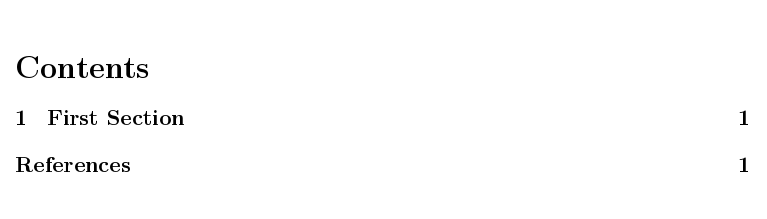
\includegraphics[width=0.70\textwidth]{gambar/Table}}
	\caption{Daftar Isi}
	\label{Daftar Isi}
\end{figure}



\vspace{\baselineskip}
\vspace{12pt}
\vspace{12pt}
	\item {\fontsize{14pt}{14pt}\selectfont \textbf{Ubah Judul Daftar Isi}}
\end{itemize}\par

\vspace{\baselineskip}
\noindent Judul default untuk daftar isi adalah "Isi", ini bisa diubah menjadi apapun yang Anda butuhkan.\par
\vspace{\baselineskip}

\noindent baris $\setminus$ renewcommand * $\setminus$ contentsname $ \{ $Summary$ \} $ akan menulis "Ringkasan" alih-alih nilai default. Jika Anda menggunakan paket babel untuk dukungan bahasa internasional, perintah tersebut harus ditempatkan di dalam tanda kurung.\par
\vspace{\baselineskip}

\noindent $\setminus$ addto $\setminus$ capionsenglish $ \{ $$ \} $\par

\vspace{\baselineskip}
\noindent Alih-alih bahasa inggris di $\setminus$ captionenglish tuliskan nama bahasa yang Anda tetapkan di babel.\par


\noindent \hspace*{0.5in}$\setminus$documentclass$ \{ $article$ \} $\par

$\setminus$usepackage[utf8]$ \{ $inputenc$ \} $\par

$\setminus$title$ \{ $Sections and Chapters$ \} $\par

$\setminus$author$ \{ $Gubert Farnsworth$ \} $\par

$\setminus$date$ \{ $ $ \} $\par
\vspace{\baselineskip}
$\setminus$renewcommand*$\setminus$contentsname$ \{ $Summary$ \} $\par

$\setminus$begin$ \{ $document$ \} $\par

$\setminus$maketitle\par

$\setminus$tableofcontents\par

$\setminus$section$ \{ $Introduction$ \} $\par
\vspace{\baselineskip}
This is the first section.\par

\vspace{\baselineskip}
Lorem~ ipsum~~dolor~ sit  amet,~~consectetuer~ adipiscing  elit. Etiam~ lobortisfacilisis~sem.  Nullam nec~mi et neque pharetra sollicitudin.  Praesent imperdietmi nec ante. Donec ullamcorper, felis non sodales...\par


\vspace{\baselineskip}
$\setminus$addcontentsline$ \{ $toc$ \} $$ \{ $section$ \} $$ \{ $Unnumbered Section$ \} $\par

$\setminus$section*$ \{ $Unnumbered Section$ \} $\par

\vspace{\baselineskip}
Lorem ipsum dolor sit amet, consectetuer adipiscing elit. Etiam~lobortis facilisissem.  Nullam nec~mi et neque pharetra sollicitudin.  Praesent imperdiet mi necante...\par


\vspace{\baselineskip}
$\setminus$section$ \{ $Second Section$ \} $\par


Lorem ipsum dolor sit amet, consectetuer adipiscing elit. Etiam~lobortis facilisissem.  Nullam nec~mi et neque pharetra sollicitudin.  Praesent imperdiet mi necante...\par




\noindent  \hspace*{0.5in}$\setminus$end$ \{ $document$ \} $\par

